% Results

Here I expect to showcase lots of nice figures and data to show how well the neural network works

\section{Training with Simulation Data}

\begin{figure}
    \centering
    \includegraphics[width=\linewidth]{Chapters/Figures/pa_train-test (3).png}
    \caption{One version of the neural network has four output nodes: one for MSD, Sigma, Mean, and Kurtosis. Sigma is just the square root of the MSD and was included during training affirm the patterns recognized by the network.}
    \label{fig:train-test-split-all4}
\end{figure}

\section{Experimental Data} \label{ch:results}
Training the neural network entirely on simulation data and then making predictions on experimental data is unlikely to provide quality results. 


\begin{figure}
    \centering
    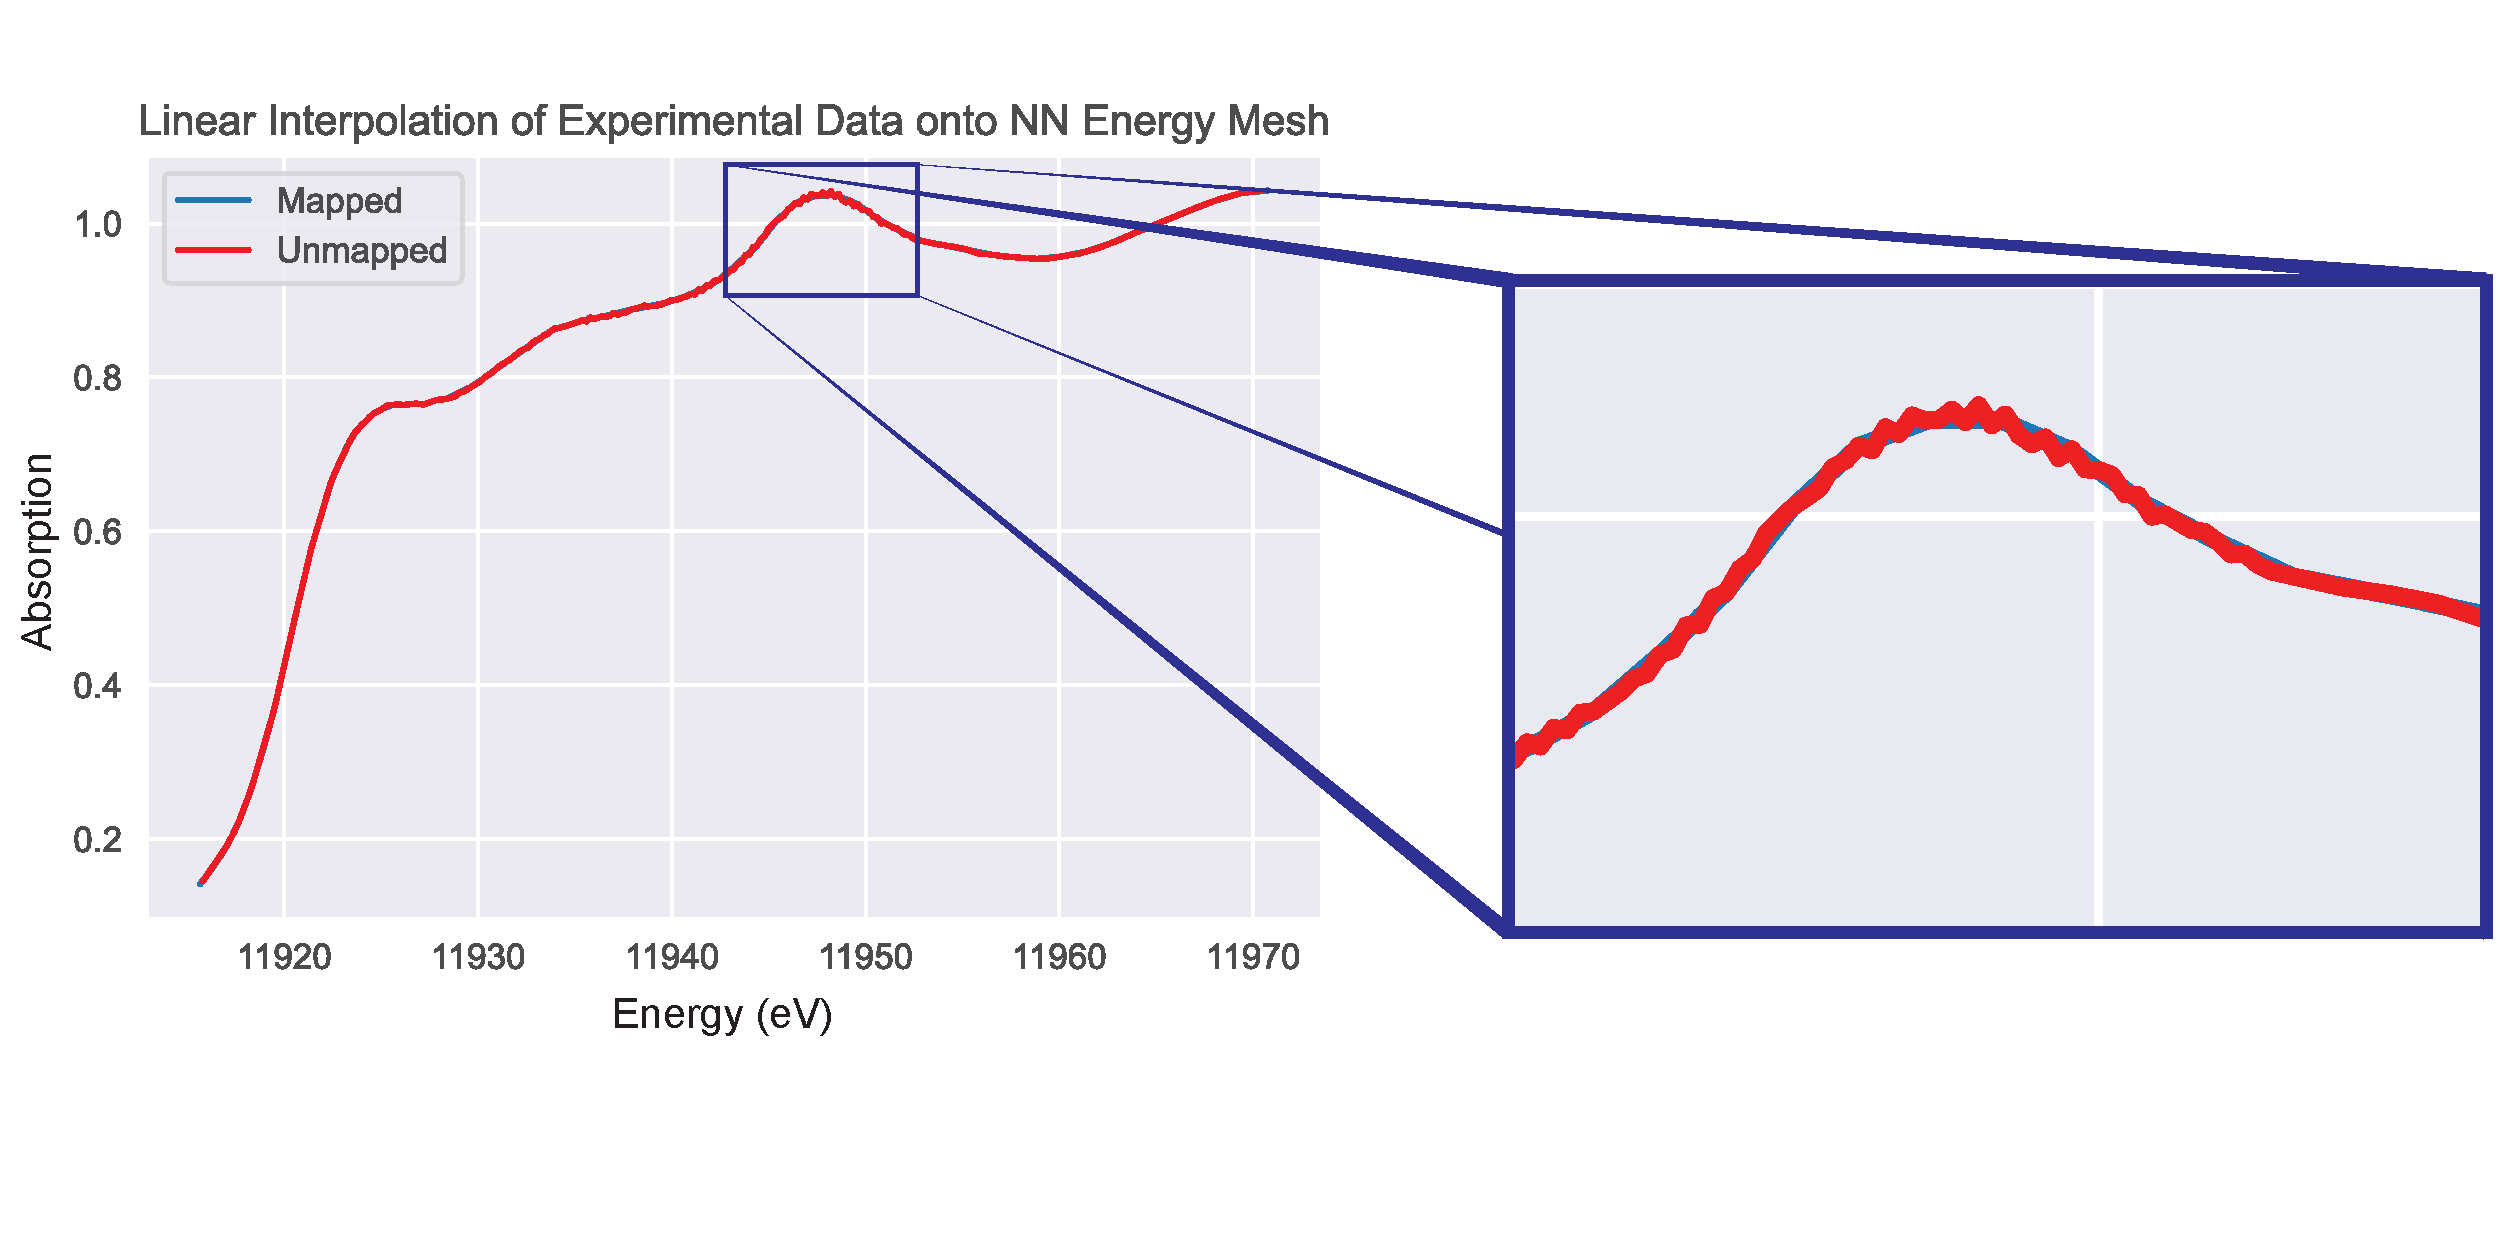
\includegraphics[width=\linewidth]{Chapters/Figures/quality-of-interpolation-figure.pdf}
    \caption[Experimental Data Interpolation]{The experimental data is measured as a function of different energy values than the ones on which the neural network is trained. Consequently, the experimental spectrum must be mapped onto the proper energy mesh via linear interpolation.}
    \label{fig:interpolation}
\end{figure}

\subsection{Data Augmentation}

\begin{figure}
    \centering
    \includegraphics[width=\linewidth]{Chapters/Figures/data-aug-shift-pt75wieght.pdf}
    \caption[Data Augmentation: Horizontal Shift]{...}
    \label{fig:data-aug-hor}
\end{figure}
